\documentclass[aspectratio=1610]{beamer}
\usetheme{boxes}
\usecolortheme{crane}
\usepackage{amsmath,amsfonts}
\usepackage{algpseudocode}
\usepackage{multicol}
\usepackage{pgfplots}
\pgfplotsset{compat=1.15}
\usepackage{mathrsfs}
\usetikzlibrary{arrows}
\usepackage{listings}
\lstset{
  language=Python,
  columns=flexible,
}

\usepackage{array}

\newenvironment{hashtable}[1][]
  {\begin{tabular}[#1]{
     @{}
     > {\small} r <{\normalsize~\rlap{\fbox{\strut~~}}$~~\rightarrow$~}
     @{} l @{}}}
  {\end{tabular}}


%-------------------------------------------------------------------
%	 TITLE SLIDE
%-------------------------------------------------------------------


\begin{document}

% -------------------------------------------------------------------
% Lesson 3
% -------------------------------------------------------------------
\section{Data Structures and Algorithms}

\begin{frame}
\begin{center}
\Huge Lesson 3\\~\\
\textbf{Data Structures and Algorithms DSA}
\end{center}
\end{frame}


\begin{frame}
\frametitle{Lesson 3}

\huge In this lesson we will talk about:
\begin{itemize}
	\item \alert{data structures}
	\item \alert{algorithm design}
	\item \alert{algorithm efficiency}
	\item \alert{searching and sorting algorithms}
\end{itemize}
\end{frame}


\begin{frame}{Lesson 3}{}
\begin{center}
\Huge \textbf{Data Structures}
\end{center}
\end{frame}


\begin{frame}{Lesson 3}{}
\Huge{What is a data structure?}\\~\\
\includegraphics[scale=0.80]{Images/ds}
\end{frame}


\begin{frame}{Lesson 3}{}
\LARGE
\textbf{Data Structures}\\~\\
\begin{itemize}
    \item How do we \textbf{organize} data
    \item For a very \textbf{efficient} access
\end{itemize}

It's a collection of data values, and the relationships among these values
\end{frame}


\begin{frame}{Lesson 3}{}
\LARGE
\textbf{Data Structures}
\begin{center}
\includegraphics[scale=0.80]{Images/data_structures}
\end{center}
\end{frame}



\begin{frame}
\frametitle{Lesson 3}
\LARGE 
\textbf{Linear Data Structures: Arrays, Queues, Stacks}\\~\\
\begin{itemize}
	\item Elements are arranged sequentially, one after the other
	\item The first element added will be the first one to be accessed or removed, and the last element added will be the last one to be accessed or removed
	\item Can have either fixed or dynamic sizes
	\item Offer very efficient data access
\end{itemize}
\end{frame}


\begin{frame}
\frametitle{Lesson 3}
\LARGE 
\textbf{Non-linear Data Structures: Trees, Graphs}\\~\\
\begin{itemize}
	\item Elements are arranged hierarchical
	\item We can’t traverse all the elements in a single run only
	\item There are multiple levels which we must traverse
	\item It is more difficult to implement
\end{itemize}
\end{frame}


\begin{frame}{Lesson 3}{}
\LARGE
\textbf{Data structures}
\begin{itemize}
    \item Sets
    \item Arrays and Matrices
    \item Stacks
    \item Queues
    \item Linked lists
    \item Trees
    \item Graphs
\end{itemize}
\end{frame}


\begin{frame}{Lesson 3}{}
\begin{center}
\Huge Sets
\end{center}
\end{frame}


\begin{frame}{Lesson 3}{Sets}
\LARGE
\textbf{Sets}\\~\\
A set is usually a \textbf{collection} of different things, fixed in size. Sets can also change size, usually when an algorithm will perform modifications against the set. We call these dynamic sets. These sets can change in size, grow or shrink, basically change over the time.
\end{frame}


\begin{frame}{Lesson 3}{Sets}
\Huge{But what is a set?}\\~\\
\end{frame}


\begin{frame}{Lesson 3}{Sets}
\LARGE
\textbf{Sets}\\~\\
The basic, fundamental data structure: \{1,2,4,51,9\}
\begin{itemize}
    \item mathematical set
    \item unchanging, unique elements, no duplicates
    \item contains a fixed number of elements: finite set
    \item or it can contain an infinite number of elements
\end{itemize}

\end{frame}


\begin{frame}{Lesson 3}{Sets}
\LARGE
\textbf{For example a set of polygons}
\begin{center}
\includegraphics[scale=0.10]{Images/set}
\end{center}
\end{frame}


\begin{frame}{Lesson 3}{Sets}
\LARGE
\textbf{Sets}\\~\\
A set is a \textbf{mathematical model} of a collection of different things. A set contains elements or members, which can be mathematical objects of any kind numbers, symbols, points in space, lines, other geometrical shapes, variables, or even other sets.

\end{frame}


\begin{frame}{Lesson 3}{Sets}
\LARGE
\textbf{Sets, examples}\\~\\
\begin{itemize}
    \item \{white, blue, red, yellow\}
    \item The empty set \{\}
    \item Natural numbers: $\mathbb{N} = \{0, 1, 2, 3, \ldots\}$
    \item Natural numbers except 0: $\mathbb{N^*} = \{1, 2, 3, \ldots\}$
    \item Integers: $\mathbb{Z} = \{\ldots, -3, -2, -1, 0, 1, 2, 3, \ldots\}$
    \item Positive integers: $\mathbb{Z_+} = \{0, 1, 2, 3, \ldots\}$
\end{itemize}
\end{frame}



\begin{frame}{Lesson 3}{Sets}
\LARGE{\textbf{\{1,2,3,4\}}}\\~\\
\LARGE
Defines a list of elements, using a simple enumeration notation (Roster notation) between curly brackets, separated by commas.
\end{frame}


\begin{frame}{Lesson 3}{Sets}
\LARGE
\textbf{Basic Operations on Sets}\\~\\
\begin{itemize}
    \item Insert - add a new element to a set
    \item Delete - remove an element from a set
    \item Test - if element X belongs to a set or not 
\end{itemize}

A dynamic set which supports all these basic operations: \textbf{a dictionary} 
\end{frame}


\begin{frame}{Lesson 3}{Sets}
\begin{center}
\includegraphics[scale=0.45]{Images/numbers3}
\end{center}
\end{frame}


\begin{frame}{Lesson 3}{Sets}
\begin{center}
\includegraphics[scale=0.14]{Images/NZQRC}
\end{center}
\end{frame}


\begin{frame}{Lesson 3}{Sets}
\LARGE
\textbf{Advantages}\\~\\
Perform operations on a collection of elements in a very \textbf{efficient} and \textbf{organized} manner
\end{frame}


\begin{frame}{Lesson 3}{Sets}
\LARGE
\textbf{Conclusions}\\~\\
Sets are basic, fundamental data structures, with:
\begin{itemize}
    \item unique elements
    \item no duplicates
    \item unchanging 
    \item fixed or infinite number of elements
\end{itemize}

\end{frame}


\begin{frame}{Lesson 3}{Sets}
\LARGE
\textbf{Im confused. Does it mean a set is similar to a Python set? Or what is the difference?}
\end{frame}


\begin{frame}{Lesson 3}{Sets}
\LARGE
\textbf{Sets vs. Python Set}\\~\\
In computer science (CS), a set is an abstract data type that can store unique values, without any particular order. It is a computer implementation of the mathematical concept of a finite set.
\end{frame}



\begin{frame}{Lesson 3}{Sets}
\LARGE
\textbf{Mathematical vs. Python Sets}\\~\\
\begin{itemize}
    \item Mathematical finite set: \{1,2,3,4\}
    \item Python set: S = \{1,2,3,4\}
\end{itemize}
\end{frame}



% %%%%%%%%%%%%%%%%%%%%%%%%%%%%%%%%%%%%%%%%%%%%%%%%%%%%
% Arrays
% %%%%%%%%%%%%%%%%%%%%%%%%%%%%%%%%%%%%%%%%%%%%%%%%%%%%

\begin{frame}{Lesson 3}{}
\begin{center}
\Huge Arrays
\end{center}
\end{frame}

\begin{frame}{Lesson 3}{Arrays}
\LARGE
\textbf{Arrays}\\~\\
In computer science, an \textbf{array} is a data structure consisting of a collection of elements, each identified by an \textbf{index} or a \textbf{key}. The simplest type of such data structure is a linear array, the one-dimensional array.
\end{frame}


\begin{frame}{Lesson 3}{Arrays}
\begin{center}
\includegraphics[scale=0.17]{Images/array2.png}
\end{center}
\end{frame}



\begin{frame}{Lesson 3}{Arrays}
\LARGE
\textbf{Arrays}\\~\\
Arrays are among the oldest and most important data structures, and are used by almost every program and programming language. They are also used to implement many other data structures, such as lists.
\end{frame}


\begin{frame}{Lesson 3}{Arrays}
\LARGE
\textbf{Arrays}\\~\\
Arrays are useful because the element indices can be computed at \alert{run time}. Among
other things, this feature allows a single iterative statement to process arbitrarily many
elements of an array. For that reason, the elements of an array data structure are required
to have the same size and should use the same data representation. 
\end{frame}



\begin{frame}{Lesson 3}{Arrays}
\LARGE
\textbf{Run-time?}\\~\\
Runtime, run time, or execution time is the final phase of a computer program's life cycle,
in which the code is being executed on the computer's central processing unit (CPU) as
machine code. In other words, "runtime" is the running phase of a program.
\end{frame}



\begin{frame}{Lesson 3}{Arrays}
\Large
\textbf{Remember this? From source code to executable}\\~\\ 
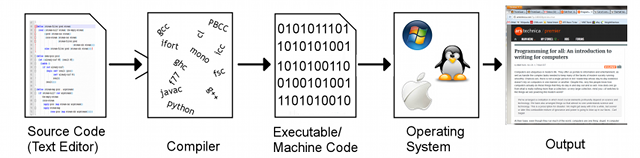
\includegraphics[scale=0.65]{Images/CompilationChain}
\end{frame}



\begin{frame}{Lesson 3}{}
\LARGE
\textbf{Basic Array Operations}\\~\\
\begin{itemize}
	\item traversal of an array
	\item access element X in an array
	\item searching element X in an array
	\item sorting an array
\end{itemize}
\end{frame}



\begin{frame}{Lesson 3}{Arrays}
\Large
\textbf{Example 1: Traversing the array A}\\~\\

\label{getArray}
\begin{algorithmic}[1]
\Procedure{getArray}{$A$} \Comment{Returns the max value in A}
\State $L\gets length(A)$
\For{\texttt{i=0 to L-1}}
    \State print $A[i]$
\EndFor
\EndProcedure
\end{algorithmic}
\end{frame}


\begin{frame}[fragile]
\LARGE
\textbf{Traversing the array}\\~\\
\Large
\begin{lstlisting}
A = [1, 2, 3, 4, 5, 6, 7,8,9]

# Traversing the array
for element in A:
    print(element, end=" ")}
\end{lstlisting}
\end{frame}



\begin{frame}[fragile]
\LARGE
\textbf{Traversing the array, version 2}\\~\\
\Large
\begin{lstlisting}
A = [1, 2, 3, 4, 5, 6, 7,8,9]

# Traversing the array
for i in range(len(A)):
    print(A[i], end=" ")
\end{lstlisting}
\end{frame}




\begin{frame}{Lesson 3}{Arrays}
\Large
\textbf{Example 2: Find the max value in the array A}\\~\\

\label{MaxArray}
\begin{algorithmic}[1]
\Procedure{MaxArray}{$A$} \Comment{Returns the max value in A}
\State $N\gets length(A)$
\State $MAX\gets A[0]$
\For{\texttt{from i=1 to N-1}}
\If {$A[i] > MAX$}
    \State \textbf{$MAX = A[i]$} \Comment{The MAX is A[i]}
\EndIf
\EndFor
\State \Return $MAX$
\EndProcedure
\end{algorithmic}
\end{frame}



\begin{frame}{Lesson 3}{Arrays}
\Large
\textbf{Example 3: Search element X in array A}\\~\\
\label{SearchArray}
\begin{algorithmic}[1]
\Procedure{SearchArray}{$A$} \Comment{Returns the max value in A}
\State $X\gets MyElement$
\State $N\gets length(A)$
\For{\texttt{from i=0 to N-1}}
\If {$X = A[i]$}
    \State \Return {$i$}  \Comment{The index for my match}
\EndIf
\EndFor
\State \Return -1 \Comment{otherwise return -1}
\EndProcedure
\end{algorithmic}
\end{frame}



\begin{frame}[fragile]
\LARGE
\textbf{Search element in array}\\~\\
\Large
\begin{lstlisting}[language=Python]
A = [1, 2, 3, 4, 5, 6, 7,8,9]

def find_element(A, n, key):
    for i in range(n):
        if A[i] == key:
            return i
    return -1

\end{lstlisting}
\end{frame}




\begin{frame}{Lesson 3}{}
\LARGE
\textbf{There are numerous applications of arrays}\\
\begin{itemize}
    \item Storing data in databases. Storing a list of customer names.  
    \item Traffic Management.Traffic management systems use arrays to track vehicles and
    their flow. By analyzing data stored in arrays, traffic control centers can implement
    efficient signal timings and manage congestion effectively.
\end{itemize}
\end{frame}



\begin{frame}{Lesson 3}{Arrays}
\LARGE
\begin{itemize}
    \item Financial Analysis. It keeps track of various financial instruments, including stocks, bonds, and mutual funds. By organizing data in arrays, companies can perform analyses and make predictions easier 
    \item Machine Learning. Machine learning algorithms often accept arrays as input, helping to train models and make predictions.
\end{itemize}
\end{frame}



% %%%%%%%%%%%%%%%%%%%%%%%%%%%%%%%%%%%%%%%%%%%%%%%%%%%%
% Matrices
% %%%%%%%%%%%%%%%%%%%%%%%%%%%%%%%%%%%%%%%%%%%%%%%%%%%%
\begin{frame}{Lesson 3}{Matrices}
\begin{center}
\Huge Matrices
\end{center}
\end{frame}


\begin{frame}{Lesson 3}{Matrices}
\LARGE
\textbf{What is a matrix?}\\~\\
In mathematics, a matrix (pl.: matrices) is a rectangular array or table of numbers,
symbols, or expressions, with elements or entries arranged in rows and columns, which is
used to represent a mathematical object or property of such an object.
\end{frame}


\begin{frame}{Lesson 3}{Matrices}
\LARGE
\textbf{Matrices}
\begin{center}
\includegraphics[scale=0.14]{Images/matrices2}
\end{center}
\end{frame}


\begin{frame}{Lesson 3}{Matrices}
\LARGE
\textbf{Matrices}
\begin{center}
\includegraphics[scale=0.10]{Images/Matrix}
\end{center}
\end{frame}


\begin{frame}[fragile]
\LARGE
\textbf{Matrix multiplication}\\~\\
   \[  \begin{bmatrix}
         0 & 1\\ 
         0 & 0 
     \end{bmatrix}
     \times
     \begin{bmatrix}
         0 & 0\\ 
         1 & 0  
     \end{bmatrix}
      =
     \begin{bmatrix}
         1 & 0\\ 
         0 & 0   
     \end{bmatrix} \] 
\end{frame}


\begin{frame}[fragile]
\LARGE
\textbf{Matrix multiplication M x N}\\~\\
\Large
    \[ \begin{bmatrix}
         a_{11} & a_{12} & \cdots & a_{1n}\\
         a_{21} & a_{22} & \cdots & a_{2n}\\ 
         \vdots & \vdots & \ddots & \vdots\\ 
         a_{m1} & a_{m2} & \cdots & a_{mn} 
     \end{bmatrix}
     \times
     \begin{bmatrix}
         b_{11} & b_{12} & \cdots & b_{1p}\\
         b_{21} & b_{22} & \cdots & b_{2p}\\ 
         \vdots & \vdots & \ddots & \vdots\\ 
         b_{n1} & b_{n2} & \cdots & b_{np} 
     \end{bmatrix}
      =
     \begin{bmatrix}
         c_{11} & c_{12} & \cdots & c_{1p}\\
         c_{21} & c_{22} & \cdots & c_{2p}\\ 
         \vdots & \vdots & \ddots & \vdots\\ 
         c_{m1} & c_{m2} & \cdots & c_{mp} 
     \end{bmatrix} \]
  \[ c_{ij}= a_{i1} b_{1j} + a_{i2} b_{2j} +\cdots+ a_{in} + b_{nj} = \sum_{k=1}^n a_{ik}b_{kj} \]
\end{frame}


\begin{frame}{Lesson 3}{Matrices}
\LARGE
\textbf{Basic Matrix Operations}\\~\\
\begin{itemize}
	\item access X element in a matrix
	\item traversal of a matrix
	\item searching a matrix
	\item sorting a matrix
\end{itemize}
\end{frame}




\begin{frame}[fragile]
\LARGE
\textbf{Accessing the elements of a matrix}\\~\\
\Large
\begin{lstlisting}[language=Python]
A = [[1, 2, 3], [4, 5, 6], [7,8,9]]

# Accessing certain elements in a matrix
print("1st element of 1st row:", A[0][0])
print("2nd element of the 2nd row:", A[1][2])
print("2nd element of 3rd row:", A[2][1])
\end{lstlisting}
\end{frame}



\begin{frame}[fragile]
\LARGE
\textbf{Traversing the matrix}\\~\\
\Large
\begin{lstlisting}[language=Python]
A = [[1, 2, 3], [4, 5, 6], [7,8,9]]

# Traversing the matrix
for row in A:
    # Traversing the matrix
    for x in row:
        print(x, end=" ")
    print()
\end{lstlisting}
\end{frame}



\begin{frame}{Lesson 3}{Matrices}
\LARGE
\textbf{There are numerous applications of matrices}\\
\begin{itemize}
    \item Encryption: Matrices encrypt data into unreadable formats and decode it for secure communication. 
    \item Computer Graphics: transformations like scaling, rotation, and translation of objects in 2D and 3D graphics
    \item Machine Learning: fundamental data structures for neural networks  
\end{itemize}
\end{frame}


\begin{frame}{Lesson 3}{Matrices}
\LARGE
\begin{itemize}
	\item Economics and Business: optimize business operations like supply chains and financial forecasting
	\item Navigation Systems: GPS systems use matrices to calculate positions, distances, and directions in 2D and 3D space.
	\item Weather Prediction: Matrices solve systems of differential equations to model and predict climate and weather patterns
\end{itemize}
\end{frame}


% %%%%%%%%%%%%%%%%%%%%%%%%%%%%%%%%%%%%%%%%%%%%%%%%%%%%
% Stacks
% %%%%%%%%%%%%%%%%%%%%%%%%%%%%%%%%%%%%%%%%%%%%%%%%%%%%
\begin{frame}{Lesson 3}{Stacks}
\begin{center}
\Huge Stacks
\end{center}
\end{frame}


\begin{frame}{Lesson 3}{Sets}
\Huge{What is a stack?}\\~\\
\end{frame}

\begin{frame}{Lesson 3}{Stacks}
\LARGE
The stack is an analogy to a set of physical items stacked one atop
another, such as a stack of plates.
\end{frame}

\begin{frame}{Lesson 3}{Stacks}
\begin{center}
\includegraphics[scale=0.23]{Images/stack}
\end{center}
\end{frame}


\begin{frame}{Lesson 3}{Stacks}
\LARGE
\textbf{Stacks}\\~\\
Stacks are collections of elements, which support two main operations:\\
\begin{itemize}
    \item \textbf{PUSH}: which adds an element to the collection 
    \item \textbf{POP}: which removes the most recent elements from the collection
\end{itemize}
\end{frame}


\begin{frame}{Lesson 3}{Stacks}
\LARGE
\textbf{Stacks}\\~\\
There might be, another operation called \textbf{PEEK}, which without
modifying the stack, return the value of the last element added.
\end{frame}


\begin{frame}{Lesson 3}{Stacks}
\LARGE
\textbf{Stacks}\\~\\
\begin{itemize}
    \item \textbf{PUSH}: which adds an element to the collection 
    \item \textbf{POP}: which removes the most recent elements from the collection
    \item \textbf{PEEK}: returns the value of the last element added
\end{itemize}
\end{frame}


\begin{frame}{Lesson 3}{Stacks}
\LARGE
\textbf{Stacks}\\~\\
The stack supports few operations. And it operates in a certain,
predefined order. The order in which an element added to or removed
from a stack is described as last in, first out,
referred to by the acronym \textbf{LIFO}
\end{frame}


\begin{frame}{Lesson 3}{Stacks}
\begin{center}
\includegraphics[scale=0.13]{Images/Lifo_stack}
\end{center}
\end{frame}


\begin{frame}{Lesson 3}{Stacks}
\LARGE
\textbf{Stacks}\\~\\
"Stacks entered the computer science literature in 1946, when
\alert{Alan Turing} used the terms "bury" and "unbury" as a means of
calling and returning from subroutines."
\end{frame}



\begin{frame}{Lesson 3}{Stacks}
{\LARGE\textbf{{Who was Alan Turing?}}}
\Large
\begin{minipage}{0.70\textwidth}
    \begin{itemize}
      \item The father of Computer Science
      \item English mathematician, computer scientist, logician, cryptanalyst
      \item Established the very first formalisation of the concepts of algorithm and computation with the Turing machine (a model of a general-purpose computer)
     \end{itemize}
  \end{minipage}
\begin{minipage}{.0\textwidth}
    % Show the image at item three and afterwards
      \begin{figure}
        \includegraphics[scale=0.28]{Images/Alan_turing}
      \end{figure}
  \end{minipage}  
\end{frame}

\begin{frame}{Lesson 3}{Stacks}
{\LARGE\textbf{{Remember this? The Turing Machine}}}\\~\\
\begin{minipage}{0.57\textwidth}
\includegraphics[scale=0.24]{Images/Turing_Machine}
\end{minipage}
\Large
\begin{minipage}{0.42\textwidth}
    \begin{itemize}
      \item Infinite tape, divided into cells with symbols
      \item A head can read/write symbols on the tape
      \item A register that stores the state of the machine
    \end{itemize}
  \end{minipage}
\end{frame}

\begin{frame}{Lesson 3}{Stacks}
\LARGE
During World War II, Turing worked for the Government Code and Cypher
School at Bletchley Park, Britain's codebreaking centre that produced
Ultra intelligence. He led Hut 8, the section responsible for German
naval cryptanalysis. Turing devised techniques for speeding the
breaking of German ciphers, including improvements to the pre-war
Polish bomba method, an electromechanical machine that could find
settings for the Enigma machine. 
\end{frame}


\begin{frame}[plain,noframenumbering]
\makebox[\linewidth]{\includegraphics[width=\paperwidth]{Images/Bombe}}
\end{frame}


\begin{frame}{Lesson 3}{Stacks}
\LARGE
\textbf{Alan Turing - the inventor of ACE}\\~\\
Automatic Computing Engine (ACE) was a British early electronic
serial stored-program computer
\end{frame}


\begin{frame}[plain,noframenumbering]
\makebox[\linewidth]{\includegraphics[width=\paperwidth]{Images/Pilot_ACE3}}
\end{frame}

\begin{frame}{Lesson 3}{}
\Huge
 Want to know more? Read about Turing. See the \textbf{Imitation Game}
 movie.
 \end{frame}
 

\begin{frame}[plain,noframenumbering]
\makebox[\linewidth]{\includegraphics[width=\paperwidth]{Images/enigma}}
\end{frame}



\begin{frame}{Lesson 3}{Stacks}
\Huge 
\textbf{Stacks}\\~\\
How can we implement a stack? 
\end{frame}


\begin{frame}{Lesson 3}{Stacks}
\LARGE
\textbf{Stacks}\\~\\
A stack can be easily implemented using an array. The first
element, usually at the zero offset, is the bottom, resulting in
array[0] being the first element pushed onto the stack and the last
element popped off. 
\end{frame}

\begin{frame}{Lesson 3}{Stacks}
\LARGE
\textbf{Stacks}\\~\\
The program must keep track of the size (length) of the stack, using a variable 
top that records the number of items pushed so far, therefore pointing to the 
place in the array where the next element is to be inserted (assuming a zero-based 
index convention).
\end{frame}



\begin{frame}{Lesson 3}{Stacks}
\LARGE
\textbf{Stacks}\\~\\
The program must keep track of the size (length) of the stack, using
a variable top that records the number of items pushed so far,
therefore pointing to the place in the array where the next element
is to be inserted (assuming a zero-based index convention).
\end{frame}


\begin{frame}[fragile]
\Large
\textbf{Stack using arrays}\\~\\
\begin{lstlisting}[language=Python]

# Create a stack. It initializes size of stack as 0 
def createStack(): 
    stack = [] 
    return stack 
\end{lstlisting}
\end{frame}

\begin{frame}[fragile]
\Large
\begin{lstlisting}[language=Python]
# Stack is empty when stack size is 0 
def isEmpty(stack): 
    return len(stack) == 0

# Add an item to stack. It increases size by 1 
def push(stack, item): 
    stack.append(item) 
    print(item + " pushed to stack ")
 \end{lstlisting}
\end{frame} 
    
    
\begin{frame}[fragile]
\Large
\begin{lstlisting}[language=Python]    
# Remove an item from stack. It decreases size by 1 
def pop(stack): 
    if (isEmpty(stack)): 
        # return minus infinite
        return str(-maxsize -1) 
    return stack.pop() 

# Return the top from stack without removing it 
def peek(stack): 
    if (isEmpty(stack)): 
        # return minus infinite
        return str(-maxsize -1)  
    return stack[len(stack) - 1] 
 \end{lstlisting}
\end{frame}


\begin{frame}[fragile]
\LARGE
\textbf{Stack using LiFoQueue}\\~\\
\Large
\begin{lstlisting}[language=Python]
from queue import LifoQueue
stack = LifoQueue()
stack.put(1)
stack.put(2)
stack.put(3)
print(stack.get()) # Prints 3
print(stack.get()) # Prints 2
\end{lstlisting}
\end{frame}



\begin{frame}{Lesson 3}{Stacks}
\LARGE
\textbf{There are numerous applications of stacks}\\
\begin{itemize}
    \item Undo mechanism in text editors
    \item Fwd and back buttons on web browsers
    \item Memory management in computer programming (static memory allocation. It can be used to keep track of functions calls)
    \item Implementing \alert{recursion}
\end{itemize}
\end{frame}



\begin{frame}{Lesson 3}{Stacks}
\Huge
 But what is recursion?
\end{frame}


\begin{frame}{Lesson 3}{Stacks}
\LARGE
\textbf{Recursion}\\
\begin{itemize}
    \item It is a programming technique, a way to program and develop a program where a function calls itself many times
    \item You take a big problem, into smaller problems, trying to apply a solution to solve the small problems
    \item You define a problem in terms of itself 
\end{itemize}
\end{frame}


\begin{frame}{Lesson 3}{Stacks}
\LARGE
\textbf{Recursion}\\~\\
You are standing in a long queue of people. You must answer, how many
people are behind you in the line?\\~\\
\large
\textbf{Note:}
One person can see only the person standing directly in front and
behind. One cannot look back and count. Each person is allowed to ask
questions from the person standing in front or behind.
\end{frame}


\begin{frame}{Lesson 3}{Stacks}
\LARGE
\textbf{Recursion}\\~\\
You look behind and see if there is a person there. If not, then you
can return the answer "0". If there is a person, repeat this step 
and wait for a response from the person standing behind. Once a
person receives a response, they add 1 and respond to the person
that asked them or the person standing in front of them.
\end{frame}


\begin{frame}{Lesson 3}{Stacks}
\Large
\textbf{Recursion example}\\~\\
\label{personCount}
\begin{algorithmic}[1]
\Procedure{personCount}{$currPerson$}
\If {$noOneBehind(currPerson) == TRUE$}
    \State \Return {$0$}
\Else { $personBehind == currPerson.checkBehind$ }
    \State \Return {$1 + \Call{personCount}{$}}    
\EndIf
\EndProcedure
\end{algorithmic}
\end{frame}



\begin{frame}{Lesson 3}{Stacks}
{\LARGE\textbf{{Thinking recursively}}}
\Large
\begin{minipage}{0.60\textwidth}
    \begin{itemize}
      \item Learning to look for big things 
      \item That are made from smaller things
    \end{itemize}
  \end{minipage}
\begin{minipage}{.0\textwidth}
    % Show the image at item three and afterwards
      \begin{figure}
        \includegraphics[scale=0.30]{Images/recursion}
      \end{figure}
  \end{minipage}  
\end{frame}



\begin{frame}{Lesson 3}{Stacks}
\LARGE
\textbf{Solving a problem recursively}\\~\\
\underline{Recursion is a function calling itself} until a generic,
base condition is true to produce the correct output. In other 
words, to solve a problem, we solve a problem that is a smaller
instance of the same problem, and then use the solution to that
smaller instance to solve the original problem.
\end{frame}



\begin{frame}{Lesson 3}{Stacks}
\LARGE
\textbf{Factorial number}\\~\\
In mathematics, the factorial of a non-negative integer 
$n!$ is the product of all positive integers less than or equal to n
\begin{equation}
n!=n \times (n-1)!
\end{equation}
\begin{equation}
n! = n \times (n-1) \times (n-2) \times \dots 3 \times 2 \times 1
\end{equation}
\end{frame}


\begin{frame}{Lesson 3}{Stacks}
\begin{center}
\includegraphics[scale=0.99]{Images/factorial2}
\end{center}
\end{frame}



\begin{frame}{Lesson 3}{Stacks}
\begin{center}
\includegraphics[scale=0.55]{Images/factorial1}
\includegraphics[scale=0.55]{Images/factorial11}
\end{center}
\end{frame}



\begin{frame}{Lesson 3}{Stacks}
\Large
\textbf{Recursion example}\\~\\
\label{factorial}
\begin{algorithmic}[1]
\Procedure{factorial}{$N$}
\If {$N == 0$}
    \State \Return {$1$}
\Else
    \State \Return {$N * \Call{factorial}{N-1}$}
\EndIf
\EndProcedure
\end{algorithmic}
\end{frame}


\begin{frame}[fragile]
\Large
\textbf{Factorial, using recursion}\\~\\
\begin{lstlisting}[language=Python]

def factorial(n):
    if n == 1:
        return 1
    else:
        return n * factorial(n-1)

print(factorial(5))
 \end{lstlisting}
\end{frame} 


\begin{frame}{Lesson 3}{Stacks}
\LARGE
\textbf{Solving a problem recursively}\\~\\
For a recursive algorithm to work, smaller subproblems must
be found and arrive at the base case. In simple words, any recursive
algorithm has two parts: the base case and the recursive structure.
\end{frame}


\begin{frame}{Lesson 3}{Stacks}
\LARGE
\textbf{The Base Case}\\~\\
The base case is a terminating condition where a function
immediately returns the result. This is the smallest version of the
problem for which we already know the solution.
\end{frame}

\begin{frame}{Lesson 3}{Stacks}
\LARGE
\textbf{The Recursive structure}\\~\\
The recursive structure is an idea to design a solution to a problem
via the solution of its smaller sub-problems, i.e., the same problem
but for a smaller input size. We continue calling the same problem
for smaller input sizes until we reach the base case of recursion.
\end{frame}



\begin{frame}{Lesson 3}{Stacks}
\LARGE
\textbf{How recursion works?}\\~\\

If we draw the flow of recursion for the factorial program, one can
find this pattern: we are calling fact(0) last, but it is returning
the value first. Similarly, we are calling fact(n) first, but it is
returning the value last. Its a Last In First Out (LIFO) order for
all recursive calls and return values.
\end{frame}



\begin{frame}{Lesson 3}{Stacks}
\LARGE
\textbf{Recursion uses Stacks behind}\\~\\
Order of recursive calls: larger problem to smaller problem
$fact(n) \rightarrow fact(n -1) \rightarrow ... 	\rightarrow fact(1) 	\rightarrow fact(0)$\\~\\
Order of return values: smaller problem to larger problem
$fact(0) \rightarrow fact(1) \rightarrow ... \rightarrow fact(n - 1) \rightarrow fact(n)$
\end{frame}


\begin{frame}{Lesson 3}{Stacks}
\LARGE
\begin{minipage}{0.50\textwidth}
    Execution call stack!
  \end{minipage}
\begin{minipage}{.0\textwidth}
    % Show the image at item three and afterwards
      \begin{figure}
        \includegraphics[scale=0.40]{Images/callstack}
      \end{figure}
  \end{minipage}  
\end{frame}



\begin{frame}{Lesson 3}{Stacks}
\LARGE
\textbf{Recursion is important!}\\
\begin{itemize}
    \item the basis for Dynamic Programming and Divide and Conquer algorithms
    \item helps in solving complex problems by breaking them into smaller subproblems
    \item fundamental to sorting, like quicksort, mergesort
    \item used in traversing trees and other complex data structures
\end{itemize}
\end{frame}



\begin{frame}{Lesson 3}{Stacks}
\Huge
Recursion vs Iteration?
\end{frame}


\begin{frame}{Lesson 3}{Stacks}
\huge
A program is called \textbf{recursive} when an entity calls itself.
A program is called \textbf{iterative} when there is a loop (or
repetition) of some sort.
\end{frame}



\begin{frame}{Lesson 3}{Stacks}
\LARGE
\textbf{Recursion}\\
\begin{minipage}{0.53\textwidth}
\begin{itemize}
    \item each function call creates a smaller problem to solve
    \item and these calls continue until reaching a basic case which is trivial to solve
\end{itemize}
  \end{minipage}
\begin{minipage}{.0\textwidth}
    % Show the image at item three and afterwards
      \begin{figure}
        \includegraphics[scale=0.30]{Images/recursion_effect}
      \end{figure}
  \end{minipage}  
\end{frame}



\begin{frame}{Lesson 3}{Stacks}
\LARGE
\textbf{Recursive function}\\
\begin{minipage}{0.60\textwidth}
\Large
\begin{itemize}
    \item \textbf{Base case} The condition under which the function stops calling itself. This prevents infinite recursion and provides a direct answer for the simplest instance of the problem.
    \item \textbf{Recursive case} The part of the function that reduces the problem into smaller instances and calls itself with small data.
\end{itemize}
  \end{minipage}
\begin{minipage}{.0\textwidth}
    % Show the image at item three and afterwards
      \begin{figure}
        \includegraphics[scale=0.26]{Images/recursion_flowchart}
      \end{figure}
  \end{minipage}  
\end{frame}



\begin{frame}[fragile]
\Large
\textbf{Recursive Factorial}\\~\\
\begin{lstlisting}
def factorial(n):
    # Base case: if n is 1 or 0, factorial is 1
    if n == 0 or n == 1:
        return 1
    # Recursive case: n * factorial of (n-1)
    else:
        return n * factorial(n - 1)
print(factorial(5))
 \end{lstlisting}
\end{frame}


\begin{frame}{Lesson 3}{Stacks}
\LARGE
\textbf{Recursion Types}\\
\begin{itemize}
    \item direct recursion
    \item indirect recursion
    \item tail recursion 
\end{itemize}
\end{frame}



\begin{frame}[fragile]
\Large
\textbf{Direct Recursion} - the simplest form of recursion. A function directly calls itself within its definition. \\~\\
\begin{lstlisting}[language=Python]
def direct_recursion(n):
    if n <= 0:
        return
    print(n)
    direct_recursion(n - 1)
 \end{lstlisting}
\end{frame} 



\begin{frame}[fragile]
\Large
\textbf{Indirect Recursion} - creates a cylces of function calls. A function calls another function, which calls the original function.\\~\\
\begin{lstlisting}[language=Python]
def functionA(n):
    if n <= 0:
        return
    print(n)
    functionB(n - 1)

def functionB(n):
    if n <= 0:
        return
    print(n)
    functionA(n - 2)
 \end{lstlisting}
\end{frame} 

    
\begin{frame}[fragile]
\Large
\textbf{Tail Recursion} - the recursive call is the last operation in the function.\\~\\
\begin{lstlisting}[language=Python]
def tail_recursion(n, aggregate=1):
    if n == 0:
        return aggregate
    return tail_recursion(n - 1, n * aggregate)
 \end{lstlisting}
\end{frame} 



\begin{frame}{Lesson 3}{Stacks}
\LARGE
\textbf{Iterative}\\
\begin{minipage}{0.60\textwidth}
\begin{itemize}
    \item a repetitive process
    \item runs a number of times until a specified condition is met
    \item or certain number of iterations have been reached
\end{itemize}
  \end{minipage}
\begin{minipage}{.0\textwidth}
    % Show the image at item three and afterwards
      \begin{figure}
        \includegraphics[scale=0.30]{Images/iteration}
      \end{figure}
  \end{minipage}  
\end{frame}



\begin{frame}{Lesson 3}{Stacks}
\LARGE
\textbf{Iterative function}\\
\begin{minipage}{0.60\textwidth}
\Large
\begin{itemize}
    \item \textbf{Initialization} Start with initializing variables or setting initial conditions required for the iterative process
    \item \textbf{Condition} Check a condition that determines whether the iteration should continue or stop
    \item \textbf{Body} Execute a set of instructions or operations that represent the core logic of the iteration. 
\end{itemize}
  \end{minipage}
\begin{minipage}{.0\textwidth}
    % Show the image at item three and afterwards
      \begin{figure}
        \includegraphics[scale=0.30]{Images/iterative_flowchart}
      \end{figure}
  \end{minipage}  
\end{frame}



\begin{frame}{Lesson 3}{Stacks}
\LARGE
\textbf{How to build an iterative function?}\\
\begin{itemize}
    \item loops: while, do-while, for loops
    \item for loop: when the number of iterations is known beforehand
    \item while loop: when the number of iterations is unknown, and the loop continues as long as a condition is true
    \item do-while loop: same as while loop but ensures that the loop is executed at least once before the condition is tested
\end{itemize}
\end{frame}



\begin{frame}[fragile]
\LARGE
\textbf{Iterative Factorial} - the iterative function to calculate the factorial\\
\Large
\begin{lstlisting}[language=Python]
def factorial(n):
    result = 1
    for i in range(1, n + 1):
        result *= i
    return result
print(factorial(5))
 \end{lstlisting}
\end{frame}



\begin{frame}{Lesson 3}{Stacks}
\LARGE
\textbf{When to use recursion vs. iteration}\\
The nature of the problem
\begin{itemize}
    \item naturally fit a recursive structure or require breaking down into smaller subproblems
    \item for loop: when the number of iterations is known beforehand
    \item use iteration for problems with a straightforward repetitive process or when the number of iterations is known beforehand
\end{itemize}
\end{frame}


\begin{frame}{Lesson 3}{Stacks}
\LARGE
\textbf{When to use recursion vs. iteration}\\
Complexity and readability
\begin{itemize}
    \item Use recursion when it simplifies the code and makes it more readable
    \item Use iteration when recursion would make the code unnecessarily complex or when avoiding the risk of stack overflow is essential
\end{itemize}
\end{frame}



\begin{frame}{Lesson 3}{Stacks}
\LARGE
\textbf{When to use recursion vs. iteration}\\
Performance consideration
\begin{itemize}
    \item Use recursion if the problem’s recursive nature allows for more elegant and maintainable code and manageable stack usage
    \item Use iteration if memory usage is a concern and the problem can be solved efficiently with loops.
\end{itemize}
\end{frame}


\begin{frame}{Lesson 3}{Stacks}
\LARGE
\textbf{Use recursion}\\
\Large
\begin{itemize}
    \item \textbf{Divide and conquer} problems like merge sort, quicksort, and binary search where the problem is divided into smaller subproblems that are solved recursively 
    \item \textbf{Tree and graph problems} Traversals (e.g., in-order, pre-order, post-order for trees) and pathfinding in graphs that naturally fit a recursive approach.
    \item \textbf{Dynamic programming} Problems like the Fibonacci sequence, where recursion with memoization simplifies the solution
    \item \textbf{Combinatorial problems} Generating permutations and combinations and solving puzzles like the Tower of Hanoi
\end{itemize}
\end{frame}



\begin{frame}{Lesson 3}{Stacks}
\LARGE
\textbf{Use iteration}\\
\Large
\begin{itemize}
    \item \textbf{Simple loops} Problems like summing a list of numbers, iterating through arrays or lists, and simple counting problems
    \item \textbf{Linear problems} Iterative solutions for problems requiring a linear scan, such as finding an array’s maximum or minimum value
    \item  \textbf{Repetitive tasks} Problems that require repeating a task a known number of times, such as printing numbers from 1 to N or iterating through data structures like arrays and linked lists.
\end{itemize}
\end{frame}


\begin{frame}{Lesson 3}{Stacks}
\begin{center}
\includegraphics[scale=0.12]{Images/Fibonacci_Spiral}
\end{center}
\end{frame}



\begin{frame}{Lesson 3}{Stacks}
\Huge 
\textbf{Fibonacci sequence}
\end{frame}


\begin{frame}{Lesson 3}{Stacks}
\LARGE
\textbf{Fibonacci sequence}\\~\\
\begin{center}
\includegraphics[scale=0.60]{Images/Fib1}
\end{center}
\end{frame}


\begin{frame}{Lesson 3}{Stacks}
\LARGE
\textbf{Fibonacci sequence}
\begin{center}
\includegraphics[scale=0.45]{Images/Fib2}
\end{center}
\end{frame}


\begin{frame}[fragile]
\Large
\textbf{Fibonacci Recursion}\\~\\
\begin{lstlisting}[language=Python]
def fibonacci_recursive(n):
    if n <= 0:
        return 0
    elif n == 1:
        return 1
    else:
        return fibonacci_recursive(n-1) + fibonacci_recursive(n-2)

# Main Code
n = 10
print(f"Recursive method: Fibonacci({n}) = {fibonacci_recursive(n)}")
 \end{lstlisting}
\end{frame} 



\begin{frame}[fragile]
\Large
\textbf{Fibonacci Iterative}\\~\\
\begin{lstlisting}[language=Python]
def fibonacci_iterative(n):
    if n <= 0:
        return 0
    elif n == 1:
        return 1
    a, b = 0, 1
    for _ in range(2, n + 1):
        a, b = b, a + b
    return b

# Main code
n = 10
print(f"Iterative method: Fibonacci({n}) = {fibonacci_iterative(n)}")
 \end{lstlisting}
\end{frame} 



\begin{frame}{Lesson 3}{Stacks}
\LARGE
\textbf{Advantages of Stacks}\\
\Large
\begin{itemize}
\item Simplicity: Stacks are a simple and easy-to-understand data structure
\item Efficiency: Push and pop operations on a stack are very fast, providing efficient access to data.
\item LIFO: Stacks follow the LIFO principle, ensuring that the last element added to the stack is the first one removed.
\item Limited memory usage: Stacks only need to store the elements that have been pushed onto them, making them memory-efficient compared to other data structures.
\end{itemize}
\end{frame}



\begin{frame}{Lesson 3}{Stacks}
\LARGE
\textbf{Disadvantages of Stacks}\\
\Large
\begin{itemize}
\item Limited access: Elements can only be accessed from the top, making it difficult to retrieve or modify elements in the middle of the stack.
\item Overflow: If more elements are pushed onto a stack than it can hold, an overflow error will occur, resulting in a loss of data.
\item No random access: Stacks do not allow for random access to elements, making them unsuitable for applications where elements need to be accessed in a specific order.
\item Limited capacity: Fixed capacity, a limitation if the number of elements that need to be stored is unknown or highly variable.
\end{itemize}
\end{frame}



% %%%%%%%%%%%%%%%%%%%%%%%%%%%%%%%%%%%%%%%%%%%%%%%%%%%%
% Queues
% %%%%%%%%%%%%%%%%%%%%%%%%%%%%%%%%%%%%%%%%%%%%%%%%%%%%
\begin{frame}{Lesson 3}{Queues}
\begin{center}
\Huge Queues
\end{center}
\end{frame}


\begin{frame}{Lesson 3}{Queues}
\LARGE
\textbf{Queues}\\~\\
A queue is a collection of entities that are maintained in
a sequence and can be modified by the addition of entities at one
end of the sequence and the removal of entities from the other end
of the sequence. 
\end{frame}


\begin{frame}{Lesson 3}{Queues}
\begin{center}
\includegraphics[scale=0.10]{Images/Queue}
\end{center}
\end{frame}


\begin{frame}{Lesson 3}{Queues}
\LARGE
By convention, the end of the sequence at which elements are added
is called \textbf{the back, tail, or rear} of the queue, and the end
at which elements are removed is called the \textbf{head or front}
of the queue, analogously to the words used when people line up to
wait for goods or services.
\end{frame}



\begin{frame}{Lesson 3}{Queues}
\LARGE
\textbf{Queues}\\~\\
The operations of a queue make it a first-in-first-out \textbf{FIFO}
data structure. In a FIFO data structure, the first element added to
the queue will be the first one to be removed.\\
A queue is an example of a linear data structure, or more abstractly
a sequential collection.
\end{frame}


\begin{frame}{Lesson 3}{Queues}
\LARGE
\textbf{Queue Properties}\\~\\
\Large
\begin{itemize}
\item \textbf{Front:} Position of the entry in a queue ready to be served, that is, the first entry that will be removed from the queue, is called the front of the queue (head of the queue)
\item \textbf{Rear:} Position of the last entry in the queue, that is, the one most recently added, is called the rear of the queue. (tail of the queue)
\item \textbf{Size:} the current number of elements in the queue 
\item \textbf{Capacity:} the maximum number of elements the queue can hold
\end{itemize}
\end{frame}


\begin{frame}{Lesson 3}{Queues}
\LARGE
\textbf{Queue Operations}\\~\\
\Large
\begin{itemize}
\item \textbf{Enqueue} — Add an element to the end of the queue
\item \textbf{Dequeue} — Remove an element from the front of the queue
\item \textbf{Is Empty} — Check if the queue is empty
\item \textbf{Is Full} — Check if the queue is full
\item \textbf{Peek} — Get the value of the front element without removing it
\end{itemize}
\end{frame}




\begin{frame}[fragile]
\Large
\textbf{Queue implements a basic FIFO queue}\\~\\
\begin{lstlisting}[language=Python]
from queue import Queue
q = Queue()
q.put(1) # Add 1 to queue
q.put(2)
q.put(3)
print(q.qsize()) # Prints 3
print(q.get()) # Prints 1
print(q.get()) # Prints 2
\end{lstlisting}
\end{frame}



\begin{frame}[fragile]
\Large
\textbf{Python Queue}\\~\\
\begin{lstlisting}[language=Python]
from queue import Queue
q = Queue()
# The key methods available are:
# qsize() - Get the size of the queue
# empty() - Check if queue is empty
# full() - Check if queue is full
# put(item) - Put an item into the queue
# get() - Remove and return an item from the queue
# join() - Block until all tasks are processed
\end{lstlisting}
\end{frame}





% %%%%%%%%%%%%%%%%%%%%%%%%%%%%%%%%%%%%%%%%%%%%%%%%%%%%
% Linked lists
% %%%%%%%%%%%%%%%%%%%%%%%%%%%%%%%%%%%%%%%%%%%%%%%%%%%%
\begin{frame}{Lesson 3}{Linked lists}
\begin{center}
\Huge Linked lists
\end{center}
\end{frame}



\begin{frame}{Lesson 3}{Linked lists}
\LARGE
\textbf{Linked Lists}\\~\\
A linked list is a linear collection of data elements where each element points to the next. 
It is a data structure consisting of a collection of nodes which together represent a sequence.
\end{frame}


\begin{frame}{Lesson 3}{Queues}
\begin{center}
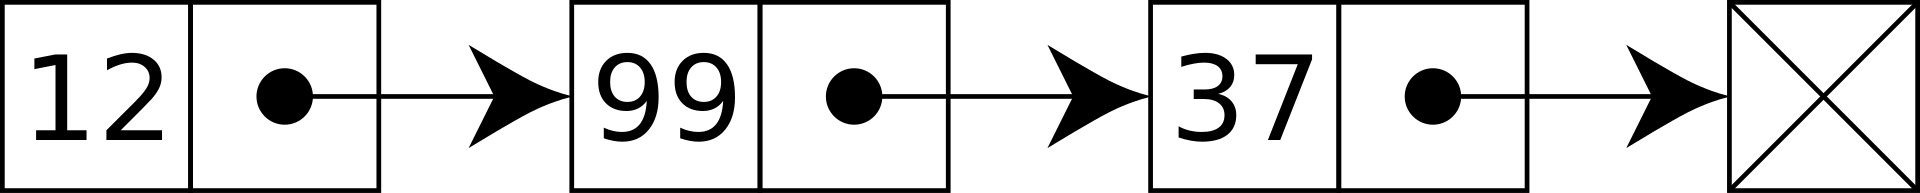
\includegraphics[scale=0.10]{Images/linked-list.png}
\end{center}
\end{frame}



\begin{frame}{Lesson 3}{Linked lists}
\LARGE
\textbf{Linked Lists}\\~\\
each node contains data, and a reference (in other words, a link) to the next node in the sequence. This structure allows for efficient insertion or removal of elements from any position in the sequence during iteration.
\end{frame}



\begin{frame}{Lesson 3}{Linked lists}
\LARGE
\textbf{Linked Lists}\\~\\
A drawback of linked lists is that data access time is linear in respect to the number of 
nodes in the list. Because nodes are serially linked, accessing any node requires that 
the prior node be accessed beforehand
\end{frame}





\begin{frame}{Lesson 3}{Linked lists}
\LARGE
\textbf{Linked Lists}\\~\\
Linked lists are among the simplest and most common data structures. They can be used to implement 
	several other common abstract data types, including stacks, queues, \alert{associative and dynamic arrays}.
\end{frame}




% %%%%%%%%%%%%%%%%%%%%%%%%%%%%%%%%%%%%%%%%%%%%%%
% Arrays
% Associative arrays
% Dynamic arrays
% %%%%%%%%%%%%%%%%%%%%%%%%%%%%%%%%%%%%%%%%%%%%%%


\begin{frame}{Lesson 3}{Linked lists}
\LARGE
\textbf{Associative Arrays}\\~\\

\end{frame}

\begin{frame}{Lesson 3}{Linked lists}
\LARGE
\textbf{Dynamic Arrays}\\~\\
Variable-size list data structure that allows elements to be added or removed. 
Dynamic arrays overcome a limit of static arrays, which have a fixed capacity that needs to be specified at allocation. 
\end{frame}


\begin{frame}{Lesson 3}{Linked lists}
\LARGE
\textbf{Associative Arrays}\\~\\
A map, symbol table, or dictionary is an abstract data type that stores a collection of (key, value) pairs, 
such that each possible key appears at most once in the collection. It supports 'lookup', 'remove', and 
'insert' operations. 
\end{frame}


\begin{frame}{Lesson 3}{Linked lists}
\LARGE
\textbf{Associative Arrays}\\~\\
\begin{hashtable}
   0 & 110 \\
   1 & 100 \\
   2 &  90 \\
   3 &  80 \\
   4 &  70 \\
   5 &  93 $\rightarrow$ 60 \\
   6 &  50 \\
   7 &  40 \\
   8 &  96 $\rightarrow$ 30 \\
   9 &  97 $\rightarrow$ 20 \\
  10 & 120 $\rightarrow$ 10
\end{hashtable}
\end{frame}





\begin{frame}{Lesson 3}{Linked lists}
\LARGE
\textbf{Linked Lists}\\~\\
The principal benefit of a linked list over a conventional array is that the list elements can be easily inserted or removed without reallocation or reorganization of the entire structure because the data items do not need to be stored contiguously in memory or on disk, while restructuring an array at run-time is a much more expensive operation.
\end{frame}




\begin{frame}{Lesson 3}{Linked lists}
\LARGE
\textbf{Linked Lists}\\~\\
 Linked lists allow insertion and removal of nodes at any point in the list, and allow doing so with a constant number of operations by keeping the link previous to the link being added or removed in memory during list traversal. 
\end{frame}



\begin{frame}{Lesson 3}{Linked lists}
\LARGE
\textbf{Linked list Operations}\\~\\
\Large
\begin{itemize}
\item \textbf{INSERT} — Add an element to the end of the queue
\item \textbf{DELETE} — Remove an element from the front of the queue
\item \textbf{TRAVERSAL} — Check if the queue is empty
\end{itemize}
\end{frame}



\begin{frame}{Lesson 3}{Linked lists}
\begin{center}
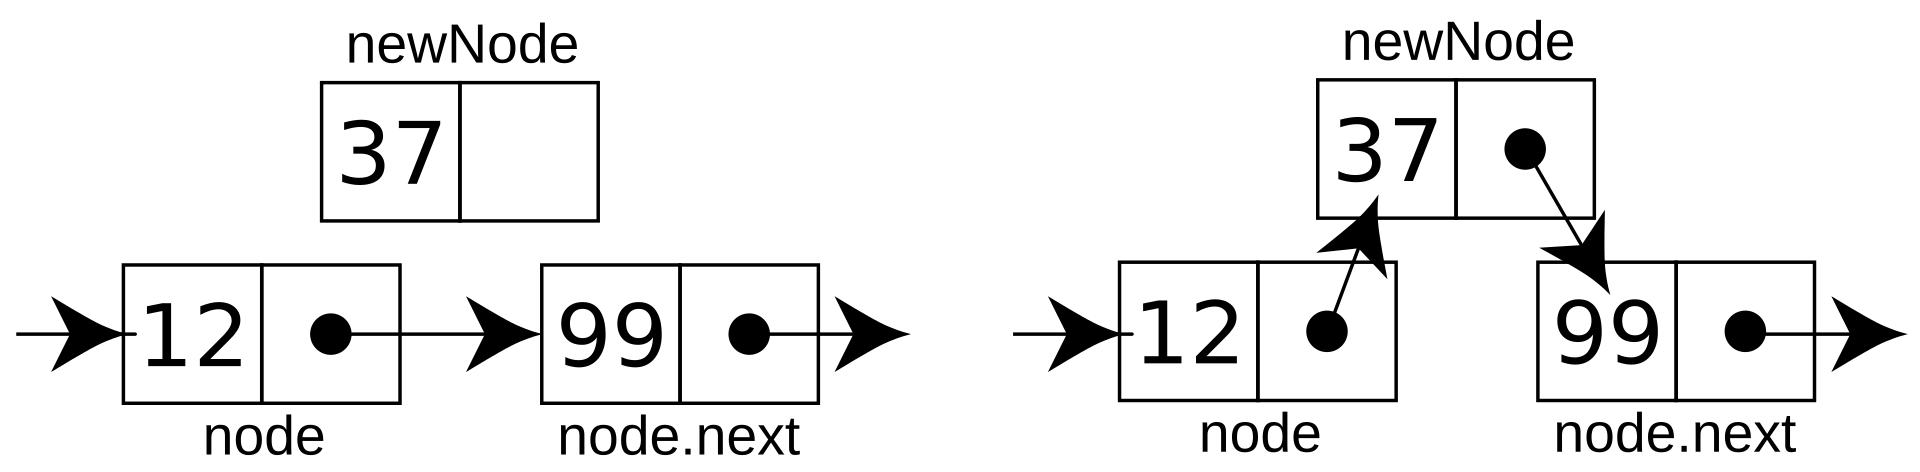
\includegraphics[scale=0.10]{Images/linkedLists-addingnode}
\end{center}
\end{frame}


\begin{frame}{Lesson 3}{Linked lists}
\begin{center}
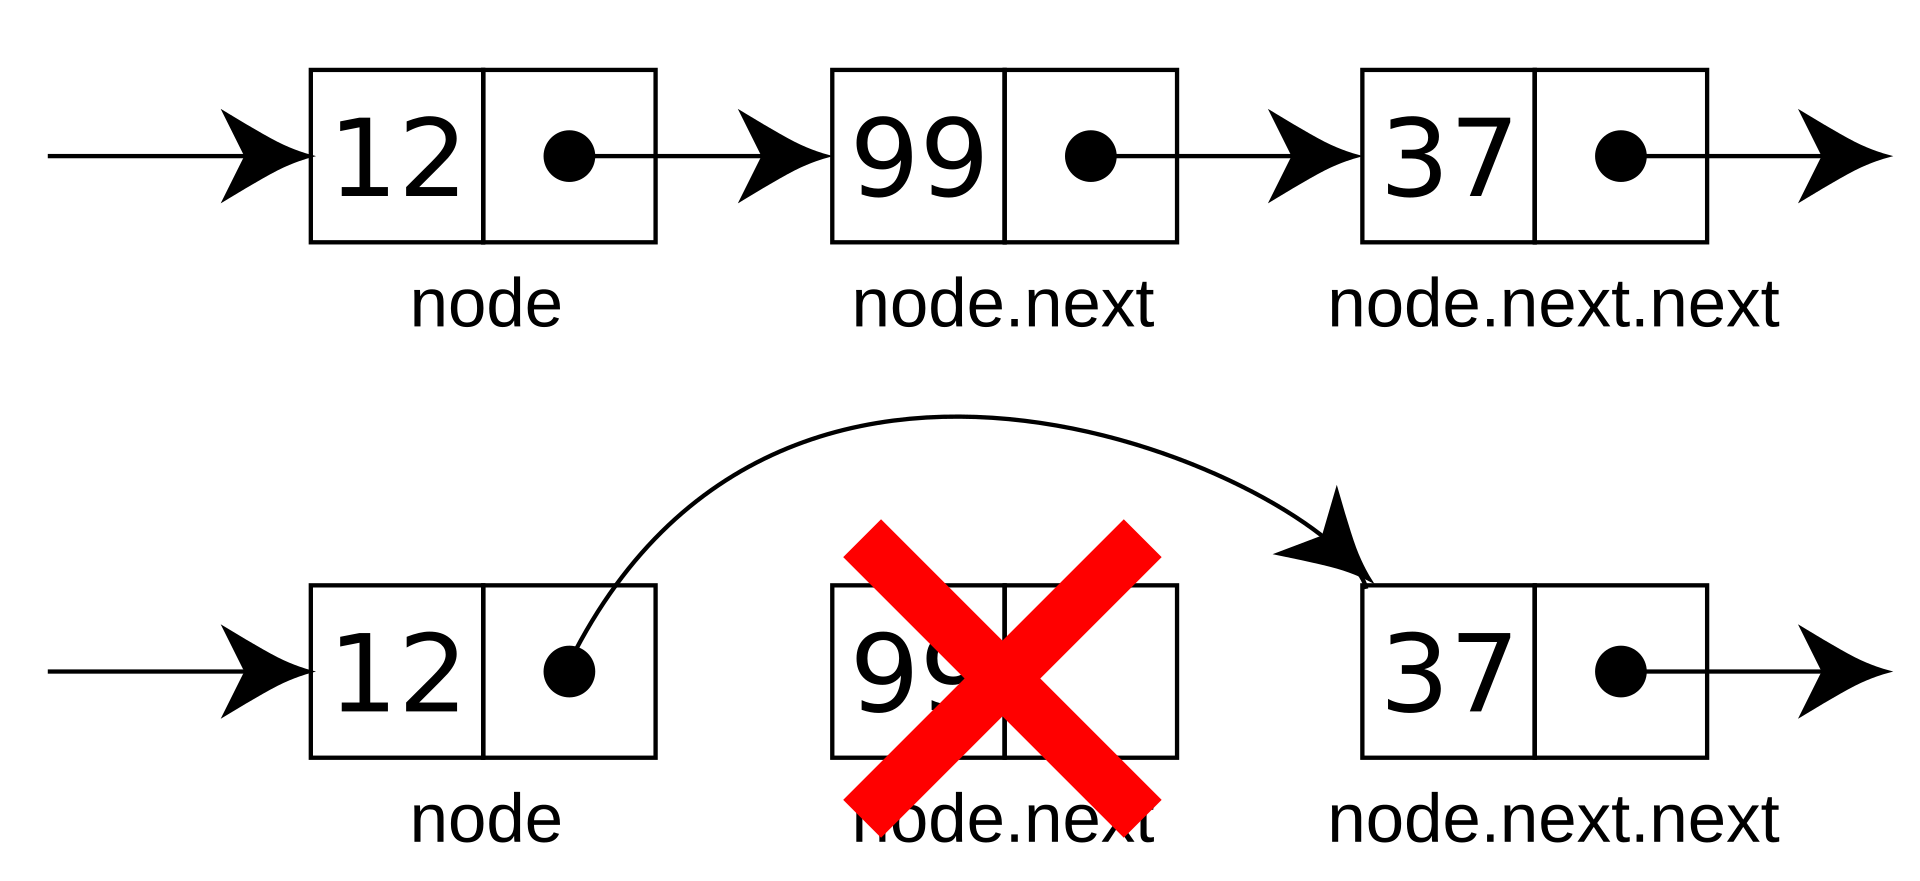
\includegraphics[scale=0.10]{Images/linkedLists-deletingnode}
\end{center}
\end{frame}


\begin{frame}{Lesson 3}{{Linked lists}
\LARGE
\textbf{Linked lists}\\~\\
\Large
\begin{itemize}
	\item \textbf{Single linked list} lists contain nodes which have a value and a next pointer
\item \textbf{Double linked list} contains nodes which inlcudes the next and previous pointer links
\item \textbf{circular linked list}  a list where the last nide has a pointer to the first node
\end{itemize}
\end{frame}



\begin{frame}{Lesson 3}{Linked lists}
\LARGE
\textbf{Single Linked list}\\~\\
\begin{center}
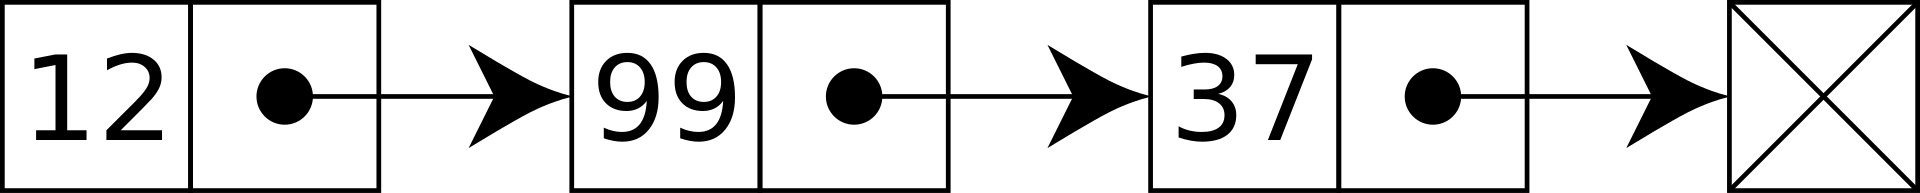
\includegraphics[scale=0.10]{Images/linked-list}
\end{center}
\end{frame}


\begin{frame}{Lesson 3}{Linked lists}
\LARGE
\textbf{Double Linked list}\\~\\
\begin{center}
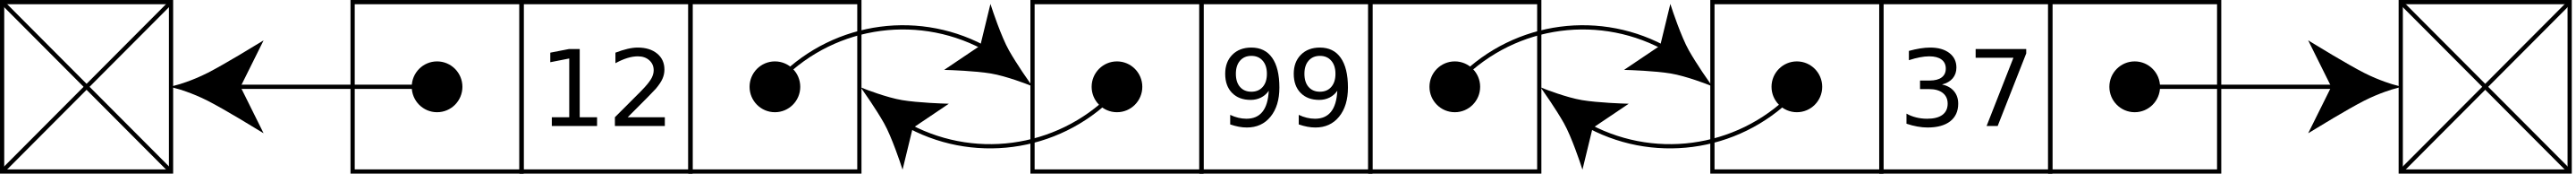
\includegraphics[scale=0.10]{Images/double-linked-list}
\end{center}
\end{frame}


\begin{frame}{Lesson 3}{Linked lists}
\LARGE
\textbf{Circular Linked list}\\~\\
\begin{center}
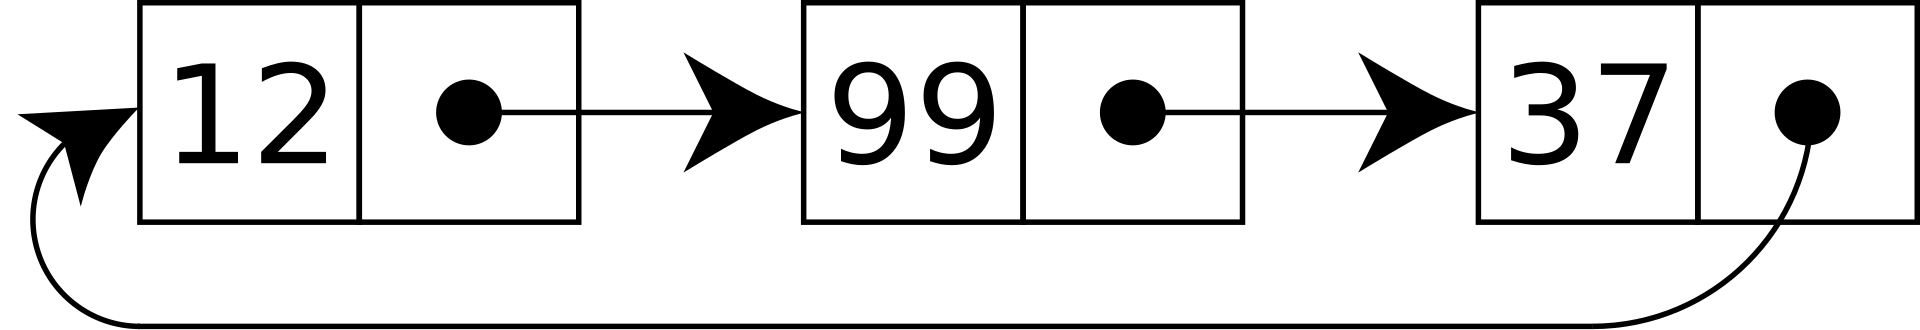
\includegraphics[scale=0.10]{Images/circular-linked-list}
\end{center}
\end{frame}





\end{document}
